% ****** Start of file apssamp.tex ******
%
%   This file is part of the APS files in the REVTeX 4.1 distribution.
%   Version 4.1r of REVTeX, August 2010
%
%   Copyright (c) 2009, 2010 The American Physical Society.
%
%   See the REVTeX 4 README file for restrictions and more information.
%
% TeX'ing this file requires that you have AMS-LaTeX 2.0 installed
% as well as the rest of the prerequisites for REVTeX 4.1
%
% See the REVTeX 4 README file
% It also requires running BibTeX. The commands are as follows:
%
%  1)  latex apssamp.tex
%  2)  bibtex apssamp
%  3)  latex apssamp.tex
%  4)  latex apssamp.tex
%
\documentclass[%
 reprint,
%superscriptaddress,
%groupedaddress,
%unsortedaddress,
%runinaddress,
%frontmatterverbose, 
%preprint,
%showpacs,preprintnumbers,
%nofootinbib,
%nobibnotes,
%bibnotes,
 amsmath,amssymb,
 aps,
%pra,
%prb,
%rmp,
%prstab,
%prstper,
%floatfix,
]{revtex4-1}

\usepackage{graphicx}% Include figure files
\usepackage{dcolumn}% Align table columns on decimal point
\usepackage{bm}% bold math
%\usepackage{hyperref}% add hypertext capabilities
%\usepackage[mathlines]{lineno}% Enable numbering of text and display math
%\linenumbers\relax % Commence numbering lines

%\usepackage[showframe,%Uncomment any one of the following lines to test 
%%scale=0.7, marginratio={1:1, 2:3}, ignoreall,% default settings
%%text={7in,10in},centering,
%%margin=1.5in,
%%total={6.5in,8.75in}, top=1.2in, left=0.9in, includefoot,
%%height=10in,a5paper,hmargin={3cm,0.8in},
%]{geometry}

\begin{document}

%\preprint{APS/123-QED}


\title{Multi-class classification on gene expression data}% Force line breaks with \\
\thanks{A footnote to the article title}%

\author{Simone Daniotti}
 \affiliation{Physics Department, University of Milan.}
 \email{daniottisimone@gmail.com}

\author{Riccardo Castelli}
  \email{riccardo.castelli3@studenti.unimi.it}
\affiliation{%
 Informatics Department, University of Milan
}%



\date{September 26, 2019}% It is always \today, today,
             %  but any date may be explicitly specified

\begin{abstract}
An article usually includes an abstract, a concise summary of the work
covered at length in the main body of the article. 
\begin{description}
\item[Usage]
Secondary publications and information retrieval purposes.
\item[PACS numbers]
May be entered using the \verb+\pacs{#1}+ command.
\item[Structure]
You may use the \texttt{description} environment to structure your abstract;
use the optional argument of the \verb+\item+ command to give the category of each item. 
\end{description}
\end{abstract}

\maketitle

\tableofcontents

\section{\label{sec:level1}Dataset description}

The dataset for this work is taken from UCI Machine Learning Repo (available at \url{https://archive.ics.uci.edu/ml/datasets/gene+expression+cancer+RNA-Seq}) \cite{Dua:2019}; this is part of the RNA-Seq (HiSeq, a tool for measuring gene expression levels) PANCAN data set. It is a collection of gene expression levels of patients having different types of tumor: BRCA(breast), KIRC(kidney), COAD(colon), LUAD(lung) and PRAD(prostate).
These data represent the quantity of gene information used in the synthesis of a functional gene product. For further information, we refer to \cite{weinstein2013cancer}.


%%%%%%%%%%%%%%%%%%%%%%%%%%%%%%%%%%%%%%%%%%%%%%%

\section{\label{sec:level1}Dataset Manipulation}


\subsection{\label{sec:level2}Preliminary manipulation}
Both dataset and labels can be downloaded in a csv ('comma separated value') format, then can be easily imported in a Pandas Dataframe (\url{https://pandas.pydata.org/}). The first column represents patient's ID: it has been removed because it is useless for our purposes.



\subsection{\label{sec:level2}Label handling}
The labels are strings representing the five types of cancer. Learning models can be created using raw features(in the case of trees and forests), using Label Encoding or One-hot Encoding.
Label Encoding creates a map between the string and an ordered sequence of natural numbers, from 0 to 4 in our case.
One-hot encoding creates a single binary label for each class, changing the task of the learning model to a multi-label problem.



\subsection{\label{sec:level2}Train and Test Set}

For training the net and then evaluating it, we split the dataset in training and test set using the Sklearn library $train\_test\_split$ (\url{https://scikit-learn.org/stable/modules/generated/sklearn.model_selection.train_test_split.html}). We set the seed of the random split and the proportions between the two sets: test set is 0.15 of the entire database.

\subsection{\label{sec:level2}Class Weighting}


%%%%%%%%%%%%%%%%%%%%%%%%%%%%%%%%%%%%%%%%%%%%%%%


\section{\label{sec:level1}Architectures}
There are lots of books reviewing these architectures and concepts. Here we refer to \cite{geron2017hands} , \cite{bishop2006pattern}
\cite{hertz1991introduction}.

\subsection{\label{sec:level2}Support Vector Machines (SVM)}

\subsection{\label{sec:level2}Decision Tree Classifier and Random Forests}

Decision Trees are versatile Machine Learning algorithms that can perform both classification and regression tasks, and even multioutput tasks. They are particularly useful in treating with complex data, such as a dataset that can hardly be represented by a vector in a multi-dimensional space: this is not our case, but we think it is useful to approach our problem with more simple models and evaluating them before \textit{deeping} in more difficult models.
Tree Classifiers have the structure of an \textit{ordered and rooted tree}. It is \textit{ordered} because the children of any internal node are numbered consecutively, and \textit{rooted} because splitting starts from only one node.
From that node, the model is built following the attribute selection measure.
Attribute selection measure is a heuristic for selecting the splitting criterion that partition data into the best possible manner.

Scikit-Learn uses the \textit{Classification And Regression Tree (CART) algorithm} to train Decision Trees.It works as follows: it first splits the training set in two subsets using a single feature k and a threshold $t_k$ . How does it choose $k$ and $t_k$? It searches for the pair $(k, t_k)$ that produces the purest subsets. The cost functions that the algorithm tries to minimize are different: most used are \textit{Gini Impurity} and \textit{Entropy}, tunable in Scikit-learn by the hyperparameter \textit{criterion}. Entropy hyperparameter measures Shannon's Entropy, a concept taken from information theory.
Each leaf of the tree corresponds to a possible classification label, so inserting datas of a patient from the root, the model $spits$ its classification. This can be a modality for building a predictor.

\begin{figure}
\centering
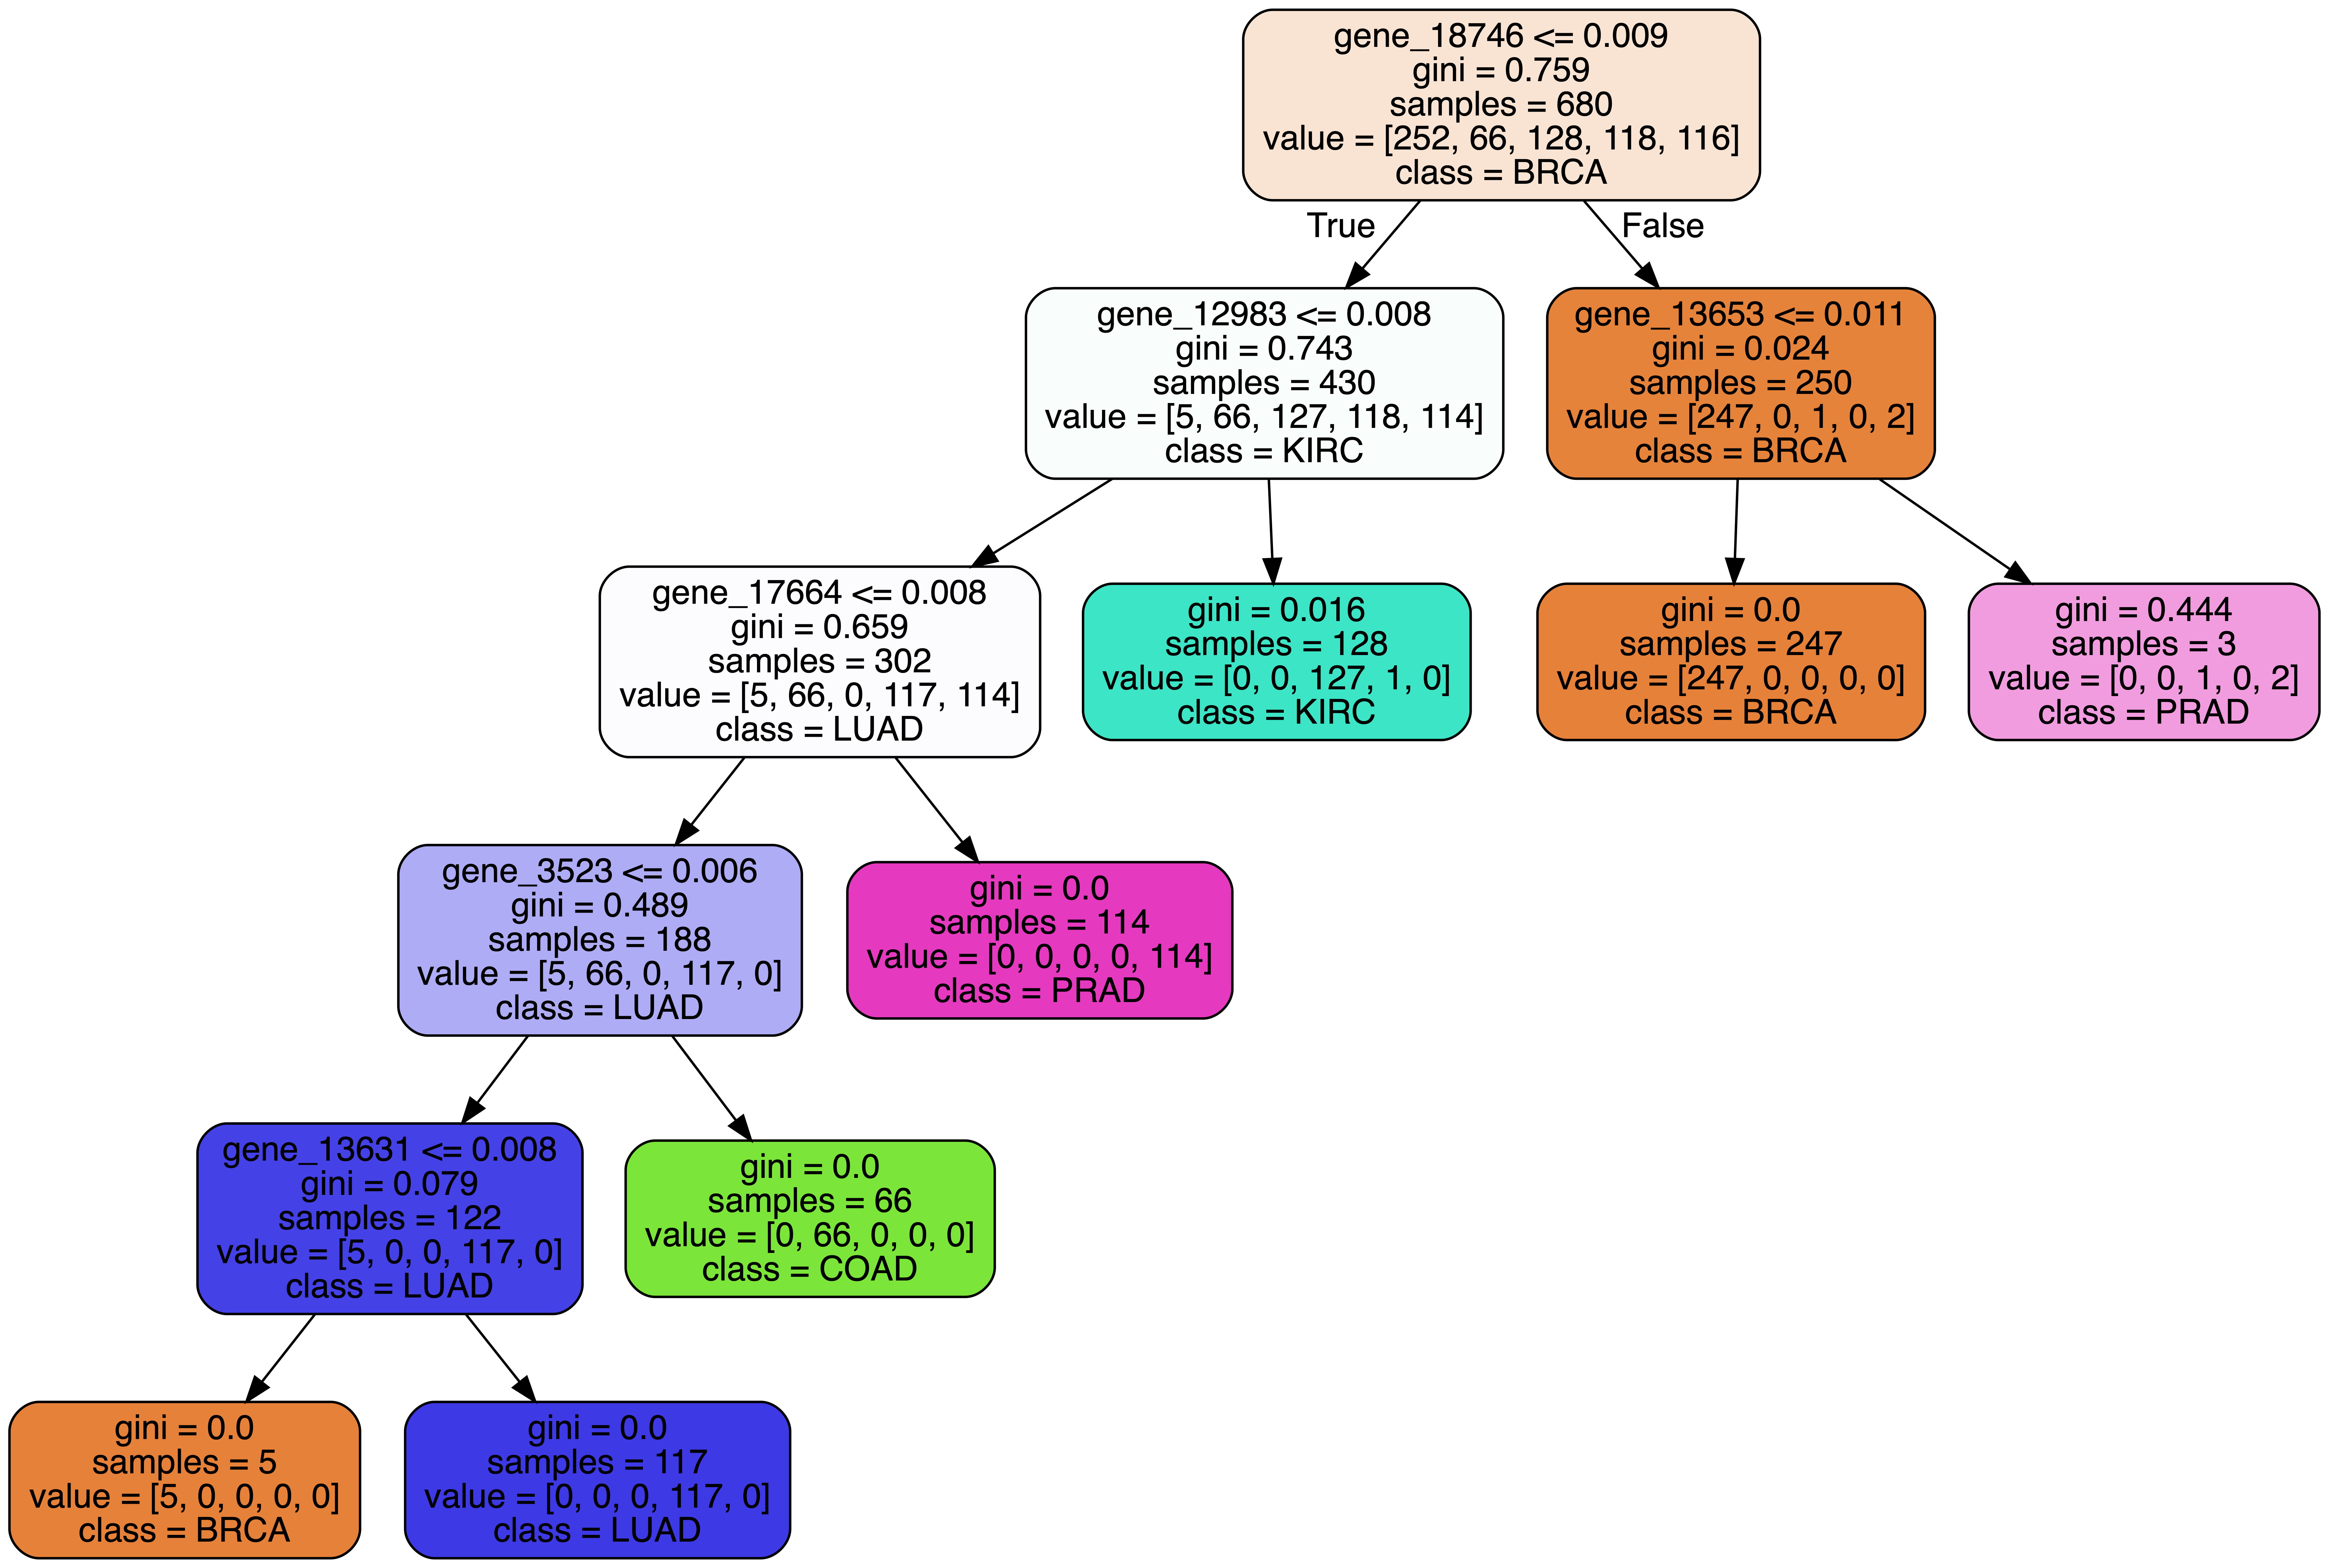
\includegraphics[width=\linewidth]{img/tree_best.png}
\caption{jnjcnkd}
\label{fig1}
\end{figure}

If you aggregate the predictions of a group of predictors (regulated by certain rules, such as majority rule..), you will often get better predictions than with the best individual predictor. A group of predictors is called an \textit{ensemble}; thus, this technique is called \textit{Ensemble Learning}, and an Ensemble Learning algorithm is called an \textit{Ensemble method}.
Training a group of Decision Tree Classifiers and gathering into one single predictor is called a \textit{Random Forest}.
The Random Forest algorithm introduces extra randomness when growing trees; instead of searching for the very best feature when splitting a node (as in the tree case), it searches for the best feature among a random subset of features. This results in a greater tree diversity.



\subsection{\label{sec:level2}Deep Learning}


%%%%%%%%%%%%%%%%%%%%%%%%%%%%%%%%%%%%%%%%%%%%%%%


\section{\label{sec:level1}Parameter optimization and Validation}

\subsection{\label{sec:level2}Cross-Validation}

\subsection{\label{sec:level2}Grid Search CV (and Random Search)}

\subsection{\label{sec:level2}Architecture setting}

\subsubsection{Parameters}

\subsubsection{Optimizers}

\subsubsection{Losses}

%%%%%%%%%%%%%%%%%%%%%%%%%%%%%%%%%%%%%%%%

\section{\label{sec:level1}Models Evaluation}

\subsection{\label{sec:level2}PCA and Permutation Importance}

\subsection{\label{sec:level2}Metrics}




%%%%%%%%%%%%%%%%%%%%%%%%%%%%%%%%
\section{\label{sec:level1}Conclusions and Outlook}


%%%%%%%%%%%%%%%%%%%%%%%%%%%%%%%%%%%




%%%%%%%%%%%%%%%%%%%%%%%%%%%%%%%%%%%%%%%%%%


\bibliography{Bibliography}
\bibliographystyle{unsrt}

\end{document}
%
% ****** End of file apssamp.tex ******
